\chapter{Spectral Rendering: What a Camera Sees}
\label{ch:xspectral}

The thesis measured beaming with the bolometric intensity, which scales as
$g^4$ and is the right quantity for flux ratios. A camera records something
else: the spectrum weighted by its colour response. This chapter derives
what that changes, documents the live renderer's colour pipeline (and the
defect found in it), and uses the result to ask what \sgra{} would look like
if it were fed by a thin disk at its measured accretion rate.

\section{A redshifted blackbody is a blackbody}
\label{sec:planckshift}

Along a light ray in vacuum $I_\nu/\nu^3$ is conserved
\citep[e.g.][]{RybickiLightman1979, MTW1973}. Light emitted at frequency
$\nu_{\rm e}$ and received at $\nu = g\nu_{\rm e}$ therefore arrives with
$I_\nu = g^3 I_{\nu/g}^{\rm (e)}$. For a blackbody emitter,
$I_\nu^{\rm (e)} = B_\nu(T) = (2h\nu^3/c^2)/(e^{h\nu/kT}-1)$, and
\begin{equation}
g^3\,B_{\nu/g}(T)
= g^3\,\frac{2h(\nu/g)^3/c^2}{e^{h\nu/(gkT)}-1}
= B_\nu(gT) .
\label{eq:planckshift}
\end{equation}
The received spectrum is exactly a blackbody at the observed temperature
$T_{\rm obs} = gT$. One lookup table of $B_\nu(T)$ through the CIE~1931
colour-matching functions \citep[fitted as in][]{WymanSloanShirley2013} then
carries everything at once: the Doppler and gravitational colour shift and the
beaming. Only the \emph{bolometric} integral of \eqref{eq:planckshift} is the
$g^4$ law, $\int B_\nu(gT)\,d\nu = \sigma (gT)^4/\pi$. A camera integrates
$B_\nu(gT)$ against its own spectral response instead, and that does not scale
as any single power of $g$.

\section{Visual versus bolometric Doppler contrast}
\label{sec:viscontrast}

The difference matters most where it is largest, between the approaching and
receding sides of the disk. Along the image major axis of the thesis'
reference view ($r_{\rm cam} = 1000\,M$, $i = 80\degr$, $\astar = 0.94$, disk
to $18\,M$; the Carter science tracer) the redshift factor of the disk ranges
from $g = \XGmin$ on the receding limb to $g = \XGmax$ on the approaching one.
\texttt{spectral\_tool} sums both the bolometric intensity and the visual
luminance $Y$ over the two halves of that axis (Fig.~\ref{fig:xcontrast}).

The bolometric ratio, $\XBoloContrast$, does not depend on the disk
temperature: every point scales by the same $T^4$. The visual ratio depends
on it strongly. For the thesis' reference temperature of 6300\,K a camera
sees the approaching side $\XVisContrastRef$ times brighter than the
receding one, \XVisBoloRatio\ times the bolometric contrast. The receding limb's light
is shifted out of the visible band onto the exponential Wien tail. For hot
disks the visible band sits on the Rayleigh--Jeans side, where
$B_\nu \propto T$, and the visual contrast drops below the bolometric one.
The two are equal at $T \approx \XContrastCrossT$\,K. The colour shifts with
them: at 6300\,K the hottest annulus seen at the extreme Doppler factors has
chromaticity $(x,y) = (\XAppChromX, \XAppChromY)$ on the approaching side, a
blue-white, and $(\XRecChromX, \XRecChromY)$ on the receding side, deep orange.

\begin{figure}
\centering
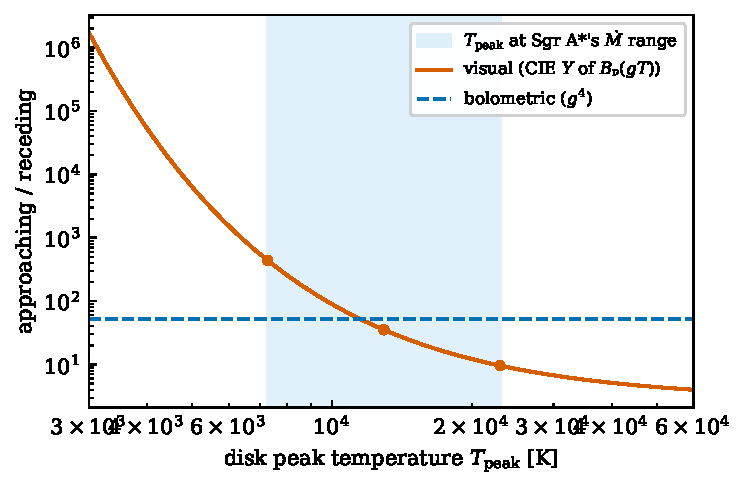
\includegraphics[width=0.75\textwidth]{figures/fig_x_contrast.pdf}
\caption{Doppler contrast between the approaching and receding halves of the
disk's major axis ($\astar = 0.94$, $i = 80\degr$, Carter tracer) as seen by a
camera (visual luminance of $B_\nu(gT)$) and bolometrically ($g^4$), versus
the disk's peak temperature. The shaded band is the peak temperature a thin
disk would have at \sgra's measured accretion rate
(\S\ref{sec:thindisk}); dots mark its three computed values.}
\label{fig:xcontrast}
\end{figure}

\section{The live colour pipeline}
\label{sec:livecolour}

The live renderer (Phases 8--15 of the thesis) coloured the disk with an
8-bit lookup table computed from the same Planck integration. Reading the
code for this extension revealed three problems:
\begin{enumerate}
\item the table stored \emph{radiance-weighted} colours,
\item it was gamma-encoded and uploaded as normalised integers,
\item the shader then multiplied by $(T_{\rm obs}/6500\,{\rm K})^4$ again.
\end{enumerate}
The temperature dependence was therefore counted twice. A 24-stop luminance
grade then mapped the result onto a narrow beige palette, which removed the
Doppler colour shift that \eqref{eq:planckshift} predicts. A separate error in
the shader's Page--Thorne flux, an extra factor $1/x^2$, made the live disk
fall off as $r^{-4}$ instead of $r^{-3}$ and run cooler than the temperature
it was given. The science path, which colours its figures with the CPU
function \texttt{planck\_to\_linear\_srgb}, was not affected.

The corrected pipeline builds a floating-point table of $B_\nu(T)$ through the
CIE curves at start-up from that same CPU function: 1024 entries,
logarithmic in $T$ from 300\,K to $10^5$\,K, normalised so that a 6500\,K
blackbody has luminance 1. The shader makes one lookup at $gT$ and nothing
else. A bolometric display mode, which shows $(gT/6500\,{\rm K})^4$ in grey,
is kept for teaching the $g^4$ law.

The validation (\texttt{compare\_live\_colour.py}) renders the thesis'
physical preset twice at identical parameters ($T_{\rm peak} = \XLiveTpeak$\,K):
once on the GPU and once with the CPU tracer and the CPU shading. Over
$\XLiveNpix$ comparable disk pixels the median luminance difference is
$|\Delta\ln Y| = \XLiveDlnYMed$ (95th percentile $\XLiveDlnYPninetyfive$\,\%),
and the median chromaticity difference is $\XLiveChromaMed$. The
approaching-to-receding luminance ratio is $\XLiveBeamCpu$ on the CPU and
$\XLiveBeamGpu$ on the GPU, a relative difference of $\XLiveBeamErr$\,\%. The
two disk footprints differ in $\XLiveMaskMismatch$\,\% of the image's pixels,
all at the one-pixel boundary between single- and double-precision tracing
(Fig.~\ref{fig:xlivecolour}).

\begin{figure}
\centering
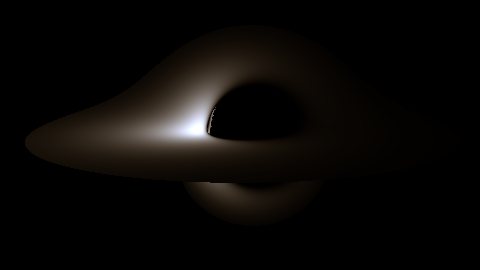
\includegraphics[width=0.49\textwidth]{figures/x_g13_cpu.png}\hfill
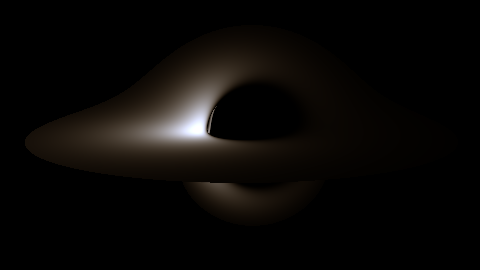
\includegraphics[width=0.49\textwidth]{figures/x_g13_gpu.png}
\caption{The physical preset ($\astar = 0.94$, $i = 80\degr$, $T_{\rm peak} =
\XLiveTpeak$\,K, linear display) rendered by the fp64 CPU reference (left) and
the live GPU path after the colour correction (right). The approaching side,
on the left, is bluer and brighter.}
\label{fig:xlivecolour}
\end{figure}

\section{The display chain}
\label{sec:display}

What a screen can show is not what the radiance image contains. Between the
two sits a display chain, applied \emph{after} the physics and switched off
completely in Science Mode, which writes the linear image with the same
transform as the CPU reference:

\begin{description}
\item[Progressive accumulation.] While the view is static, every frame adds
one jittered sample per pixel to a floating-point running mean. The jitter
follows the R2 low-discrepancy sequence \citep{Roberts2018}. Sample 0 is the
un-jittered pixel centre, so one sample reproduces the historical image
exactly.
\item[Exposure metering.] Exposure value 0 places the luminance of the
un-beamed disk at its peak temperature at display level 1, as a camera's
meter would, so disks of 7000\,K and 23\,000\,K are both well exposed.
\item[Bloom.] An energy-conserving dual-filter mip pyramid
\citep{Jimenez2014}, with a luminance-weighted first level so that single
hot pixels cannot flicker into glare.
\item[White balance and tone curve.] White-balance gains render a blackbody
of the chosen temperature neutral. A filmic curve, AgX \citep[][via the
polynomial fit of \citealt{Wrensch2023}]{Sobotka2022} or ACES
\citep{Narkowicz2016}, compresses the range while keeping hue in
overexposed regions.
\end{description}

\section{A thin disk at \sgra's real accretion rate}
\label{sec:thindisk}

The thesis' disk temperature was a display choice. Here it is computed.
Restoring $G$ and $c$ in the Page--Thorne flux \citep{PageThorne1974} gives
$F(r) = 3\mdot c^6/(8\pi G^2M^2)\,f(r)$ and $\sigma T_{\rm eff}^4 = F$. The
accretion rate of \sgra{} is bounded by the Faraday rotation of its 230\,GHz
emission to $\XMdotLow \lesssim \mdot \lesssim \XMdotHigh\,\msun\,{\rm yr}^{-1}$
\citep{Marrone2007}; see also the review by \citet{Genzel2010}. Over that
range a Novikov--Thorne disk around \sgra{} ($\astar = 0.94$) would peak at
\begin{equation}
T_{\rm peak} = \XTpeakLow\text{--}\XTpeakHigh\ {\rm K}
\qquad (\mdot = \XMdotLow\text{--}\XMdotHigh\ \msun\,{\rm yr}^{-1}),
\end{equation}
at $r = \XRpeak\,M$ ($\XTpeakMid$\,K at $\XMdotMid$). It would look
blue-white: the chromaticity at its peak moves from $(\XChromXLow,
\XChromYLow)$ to $(\XChromXHigh, \XChromYHigh)$ across the range.

Such a disk would also be far too bright. Its luminance $L = \eta\mdot c^2$,
with radiative efficiency $\eta = 1 - E_{\rm ISCO} = \XEta$ for this spin,
spans $\XLumLow$--$\XLumHigh$\,erg\,s$^{-1}$, or $\XLumEddLow$--$\XLumEddHigh$
of the Eddington luminosity ($\XLEdd$\,erg\,s$^{-1}$ at the GRAVITY mass).
\sgra{} radiates on average about $10^{-8.5}$ of its Eddington luminosity
\citep{Genzel2010}. A thin disk fed at the measured rate would therefore
outshine it by a factor $\XLumFactorLow$--$\XLumFactorHigh$. This is the
classic argument, made quantitative here, that the accretion flow of
\sgra{} is radiatively inefficient: a hot, geometrically thick, optically thin
plasma that radiates a tiny fraction of its accretion energy. That flow is
the subject of Chapter~\ref{ch:xriaf}. The thin disk survives in the renderer
as a labelled hypothetical, with its temperature computed rather than chosen
(Table~\ref{tab:xpresets}, Fig.~\ref{fig:xpresets}).

\begin{table}
\centering
\caption{The live renderer's scenes: one spacetime ($\astar = 0.94$), five
cameras and accretion rates. The thin disk is hypothetical (\S\ref{sec:thindisk});
its peak temperature follows from $\mdot$. ``Soft'' styles fade the disk's
outer rim; ``clouds'' adds an optically thin, locally thermal cloud layer
moving on the disk's own circular orbits (display only, removable).}
\label{tab:xpresets}
\small\setlength{\tabcolsep}{4pt}
% AUTO-GENERATED by scripts/make_numbers_ext.py from DiskPreset.hpp — do not edit.
\begin{tabular}{llrrrcr}
\toprule
Scene & style & $i$ [deg] & $r_{\rm cam}/M$ & $r_{\rm out}/M$ & $\dot M$ [$\msun\,{\rm yr}^{-1}$] & $T_{\rm peak}$ [K] \\
\midrule
Physical & exact & 80 & 60 & 18 & $2\times10^{-8}$ & 12\,900 \\
Earth View ($i=30\degr$) & soft & 30 & 60 & 18 & $2\times10^{-8}$ & 12\,900 \\
Close Orbit & soft, clouds & 84 & 45 & 24 & $2\times10^{-8}$ & 12\,900 \\
Low $\dot M$ & soft & 78 & 60 & 18 & $2\times10^{-9}$ & 7\,280 \\
High $\dot M$ & soft & 78 & 60 & 18 & $2\times10^{-7}$ & 23\,000 \\
\bottomrule
\end{tabular}

\end{table}

\begin{figure}
\centering
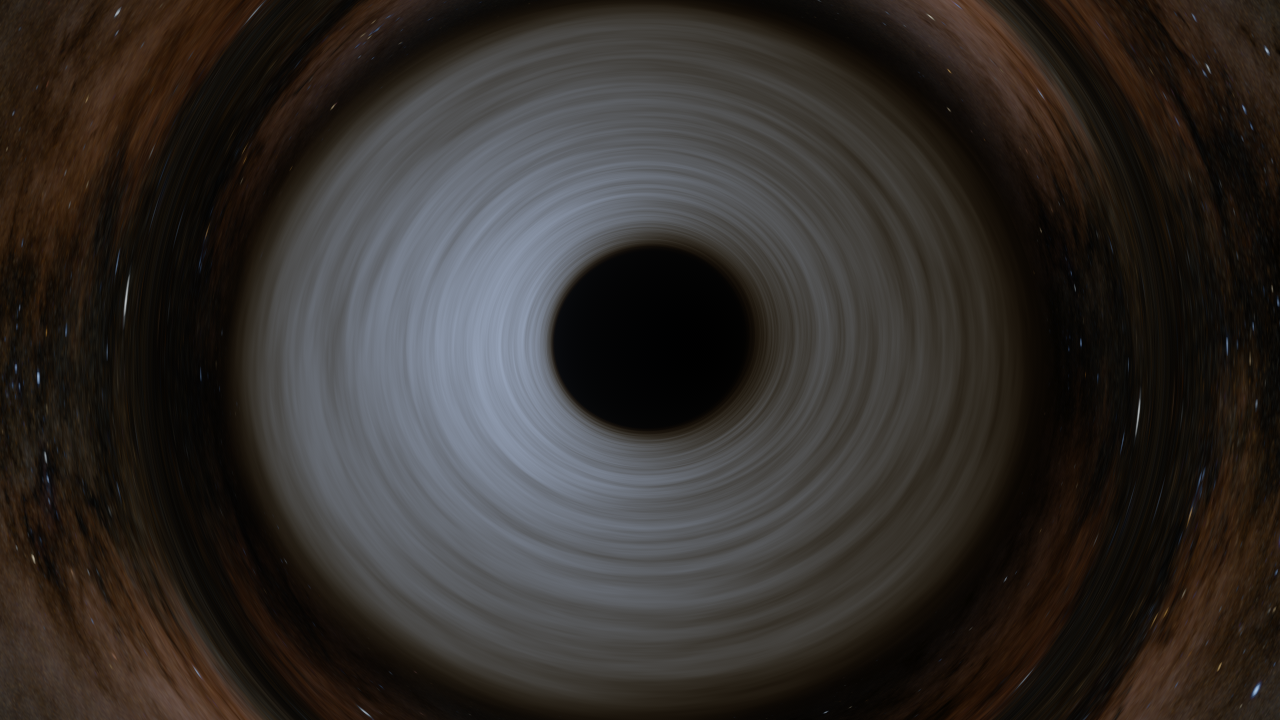
\includegraphics[width=0.49\textwidth]{figures/x_preset1_earth.png}\hfill
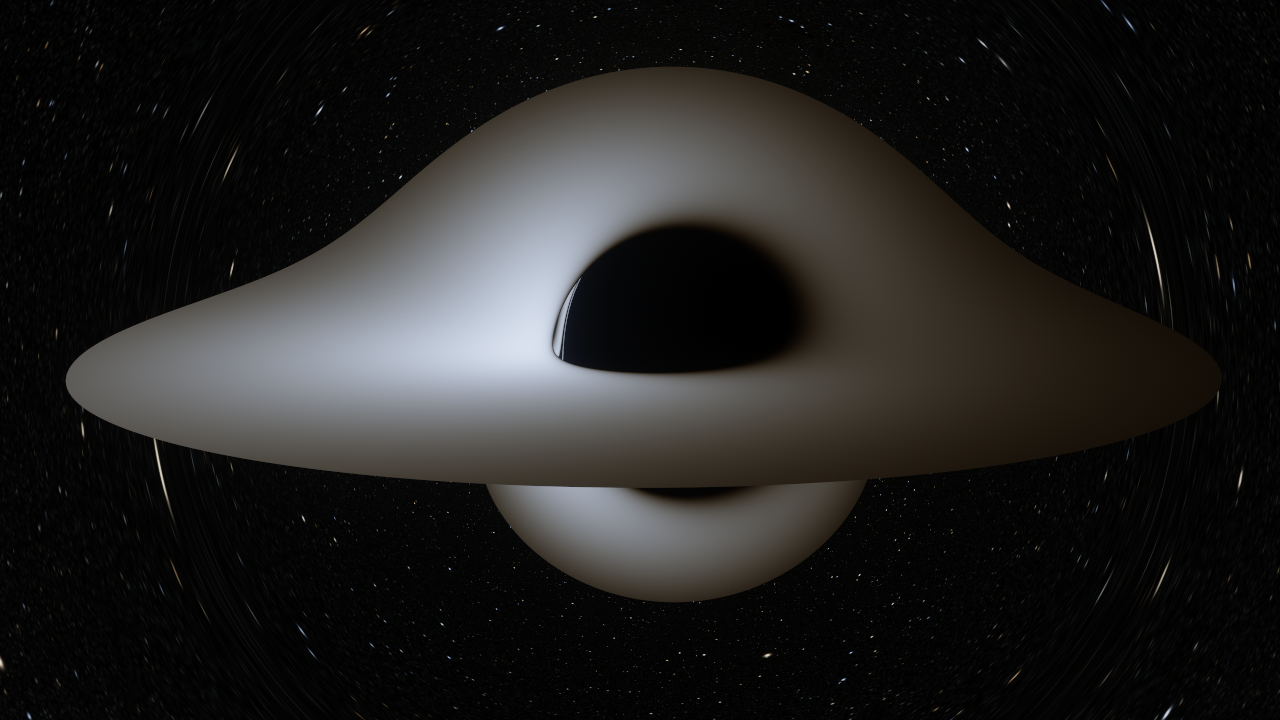
\includegraphics[width=0.49\textwidth]{figures/x_preset0_physical.png}\\[4pt]
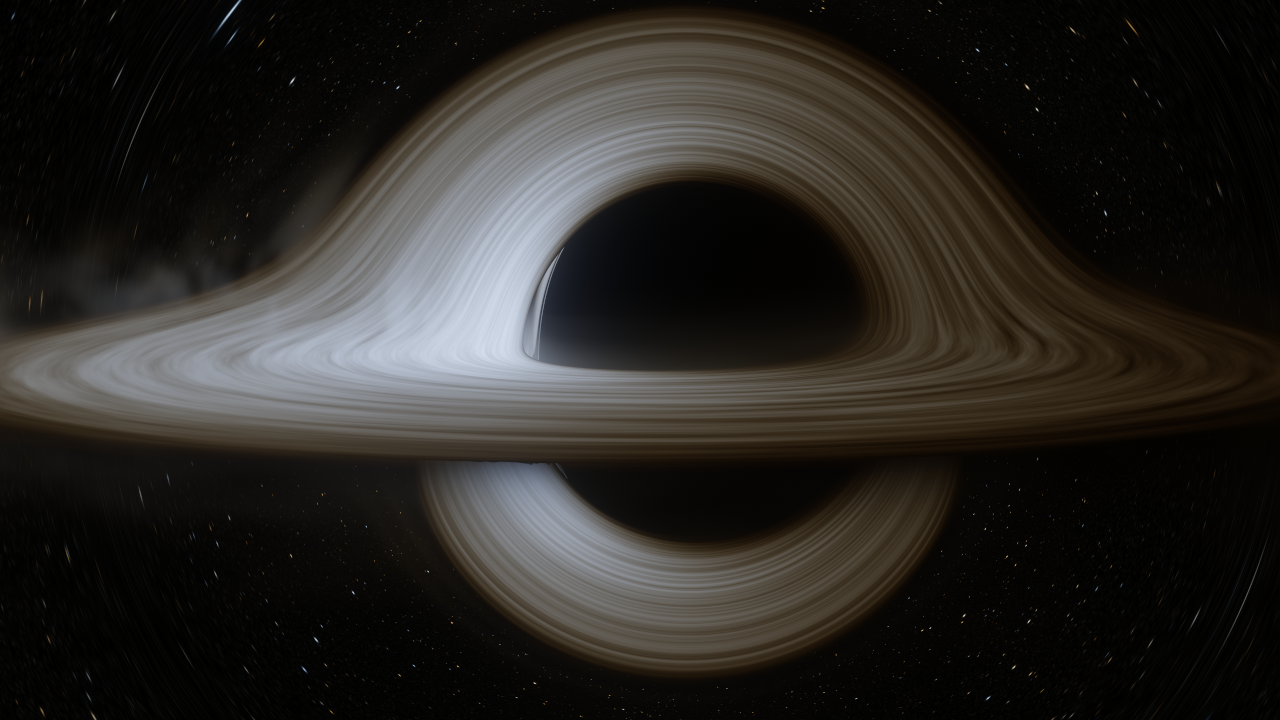
\includegraphics[width=0.49\textwidth]{figures/x_preset2_close.png}\hfill
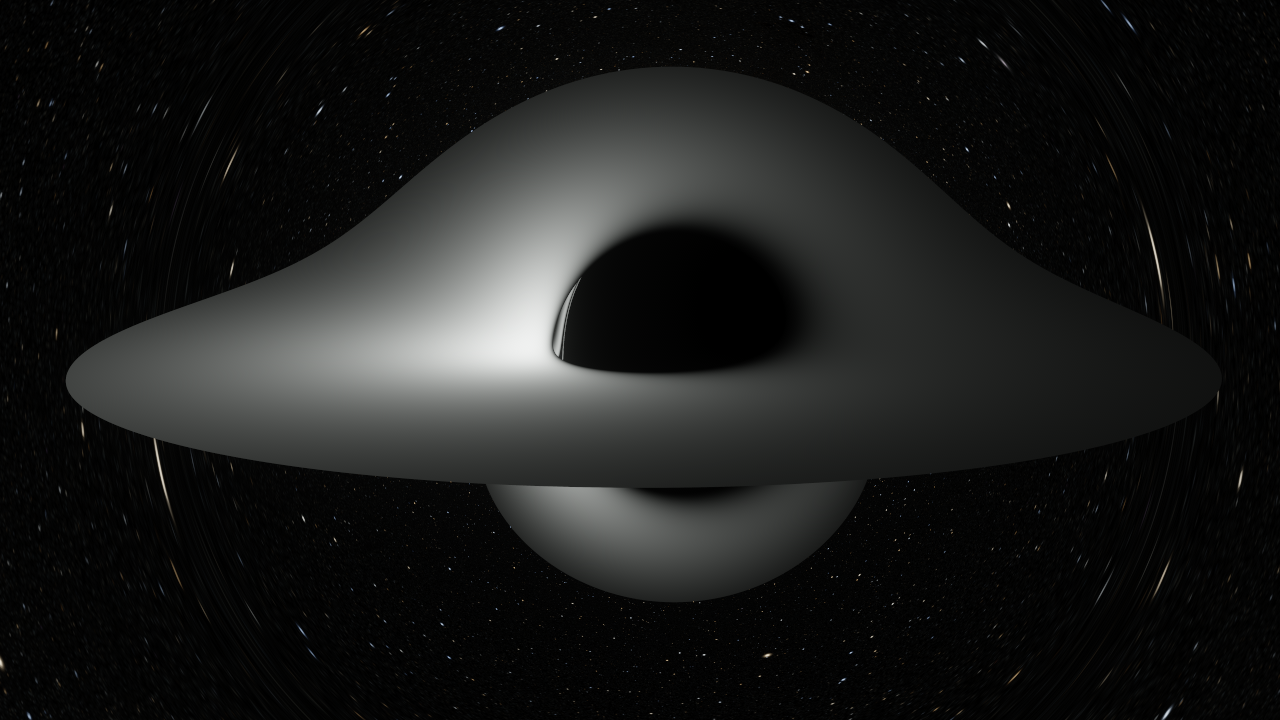
\includegraphics[width=0.49\textwidth]{figures/x_preset0_bolometric.png}
\caption{\sgra{} with a hypothetical thin disk at the computed temperature of
$\mdot = \XMdotMid\,\msun\,{\rm yr}^{-1}$. Top: the EHT viewing geometry
($i = 30\degr$, left) and the physical preset ($i = 80\degr$). Bottom left: a
close orbit with the cloud layer. Bottom right: the physical preset in the
bolometric view, which shows the $g^4$ beaming in grey. The background is the
lensed Milky Way (\S\ref{sec:sky}). Engine commands:
\texttt{scripts/render\_ext\_gallery.py}.}
\label{fig:xpresets}
\end{figure}

\section{The lensed Milky Way}
\label{sec:sky}

The thesis rendered a procedural starfield. The background is now the real
sky: the NASA SVS \emph{Deep Star Maps 2020} panorama \citep{Wright2020},
built from Gaia DR2 \citep{Gaia2018}, Hipparcos-2 and Tycho-2, in galactic
coordinates (plate carr\'ee, 8192$\times$4096). Each escaping ray reads the
map in its asymptotic direction. The texture level follows the pixel
footprint, so the dense star clouds do not alias; strongly lensed regions
alias per sample, which progressive accumulation averages away. The map is
placed with the spin axis at $i = 30\degr$ to our line of sight
\citep{EHT2022}, so a camera at that inclination sees the Galactic-Centre
star clouds behind the hole. The spin's position angle on the sky is not
constrained by current data and is set to zero, an assumption stated in the
interface.

Two caveats apply. The panorama is the sky seen \emph{from Earth}, used as a
backdrop at infinity: from the Galactic Centre, stars within a few
kiloparsecs would lie in different directions. And the map is an RGB image,
not a spectrum: when an observer's motion or gravity shifts the received
light by a factor $g$ (Chapter~\ref{ch:xobs}), each map pixel is shifted as a
6500\,K blackbody would be, $B(6500\,{\rm K}\cdot g)/B(6500\,{\rm K})$ per
channel, which gives the right sense and size of the colour and brightness
change but not a star-by-star spectrum.
